% Method figure: \input after macros.tex. Rendered by paper/figures/make_method.py (real PACO test image, pool and scores).
\begin{figure*}[t]
  \centering
  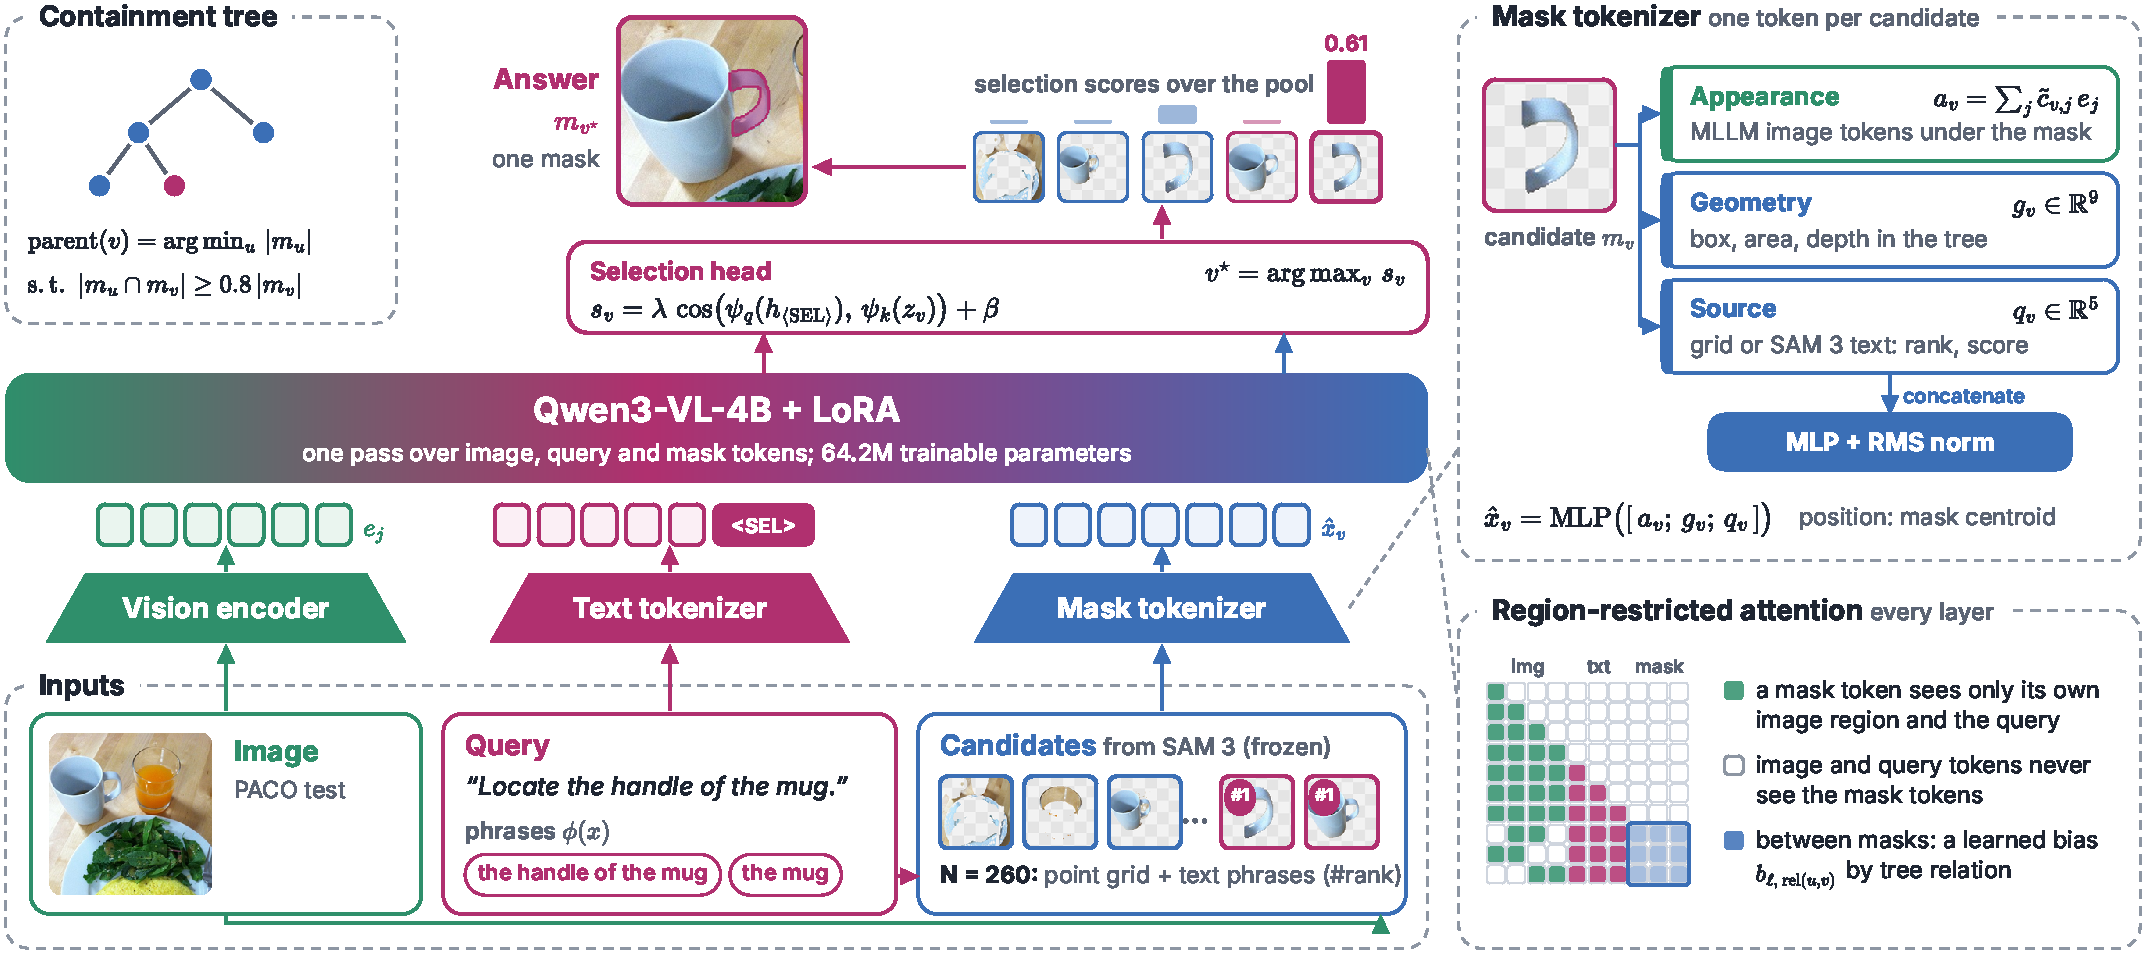
\includegraphics[width=\linewidth]{figures/method_cropped.pdf}
  \caption{\textbf{\ours{}.} A frozen SAM\,3 proposes candidate masks for the image: query-free masks from a point grid
  and the top instances for the query's own phrases. Each candidate becomes one \emph{mask token}, built like a word
  token from its content (the MLLM's own image tokens under the mask), its position (box, area, place in the
  containment tree) and its type (grid mask or SAM\,3 instance, with rank and score). Image, query and mask tokens pass
  through the MLLM once; each mask token attends to the query and to its own image region. The selection head scores
  every candidate from the \texttt{<SEL>} state, and the answer is the top-scoring mask: the MLLM never draws pixels.}
  \label{fig:method}
\end{figure*}
